\documentclass{oblivoir}
\usepackage{amsmath,amssymb,amsthm,kotex,paralist,kswrapfig,tabu}

\usepackage[skipabove=10pt,skipbelow=10pt,innertopmargin=10pt]{mdframed}

\usepackage{tabto,pifont}
\TabPositions{0.2\textwidth,0.4\textwidth,0.6\textwidth,0.8\textwidth}
\newcommand\tabb[5]{\par\bigskip\noindent
\ding{172}\:{\ensuremath{#1}}
\tab\ding{173}\:\:{\ensuremath{#2}}
\tab\ding{174}\:\:{\ensuremath{#3}}
\tab\ding{175}\:\:{\ensuremath{#4}}
\tab\ding{176}\:\:{\ensuremath{#5}}}

\usepackage{enumitem}
\setlist[enumerate]{label=(\arabic*)}

\newcounter{num}
\newcommand{\defi}[1]
{\noindent\refstepcounter{num}\textbf{정의 \arabic{num}) #1}\par\noindent}
\newcommand{\theo}[1]
{\noindent\refstepcounter{num}\textbf{정리 \arabic{num}) #1}\par\noindent}
\newcommand{\exam}[1]
{\bigskip\bigskip\noindent\refstepcounter{num}\textbf{예시 \arabic{num}) #1}\par\noindent}
\newcommand{\prob}[1]
{\bigskip\bigskip\noindent\refstepcounter{num}\textbf{문제 \arabic{num}) #1}\par\noindent}
\newcommand{\proo}
{\bigskip\textsf{증명)}\par}

\newcommand{\procedure}[1]{\begin{mdframed}\vspace{#1\textwidth}\end{mdframed}}
\newcommand{\ans}{
{\par\raggedleft\textbf{답 : (\qquad\qquad\qquad\qquad\qquad\qquad)}\par}\bigskip\bigskip}
\newcommand\an[1]{\par\bigskip\noindent\textbf{문제 #1)}\\}

\newcommand{\pb}[1]%\Phantom + fBox
{\fbox{\phantom{\ensuremath{#1}}}}

\newcommand\ba{\,|\,}

\let\oldsection\section
\renewcommand\section{\clearpage\oldsection}
\counterwithout{subsection}{section}

\newenvironment{talign}
 {\let\displaystyle\textstyle\align}
 {\endalign}
\newenvironment{talign*}
 {\let\displaystyle\textstyle\csname align*\endcsname}
 {\endalign}

\let\emph\textsf

%\usepackage{fapapersize}
%\usefapapersize{210mm,297mm,15mm,15mm,15mm,15mm}
%%%%
\begin{document}

\title{준영 : 09 모의고사(2016년 3월) 해설 및 유사문제}
\author{}
\date{\today}
\maketitle

\clearpage
%
\prob{9번}
어느 지역에서 1년동안 발생하는 규모 \(M\) 이상인 지진의 평균 발생 횟수 \(N\)은 다음 식을 만족시킨다고 한다.
\[\log N=a-0.9M\quad\text{(단, \(a\)는 양의 상수)}\]
이 지역에서 규모 \(4\) 이상인 지진이 1년에 평균 \(64\)번 발생할 때, 규모 \(x\)이상인 지진은 1년에 평균 한 번 발생한다.
\(9x\)의 값을 구하시오.
(단, \(\log2=0.3\)으로 계산한다.)
\tabb{27}{36}{45}{54}{63}

\clearpage
%
\prob{15번}
이차항의 계수가 \(1\)인 이차함수 \(y=f(x)\)의 그래프와 직선 \(y=g(x)\)가 만나는 두 점의 \(x\)좌표는 \(-1\)과 \(5\)이다.
\(h(x)=f(x)-g(x)\)라고 할 때, 함수 \(h(x)\)는 \(x=p\)에서 최솟값 \(q\)를 갖는다.
\(p+q\)의 값은?
\begin{figure}[h!]
\centering
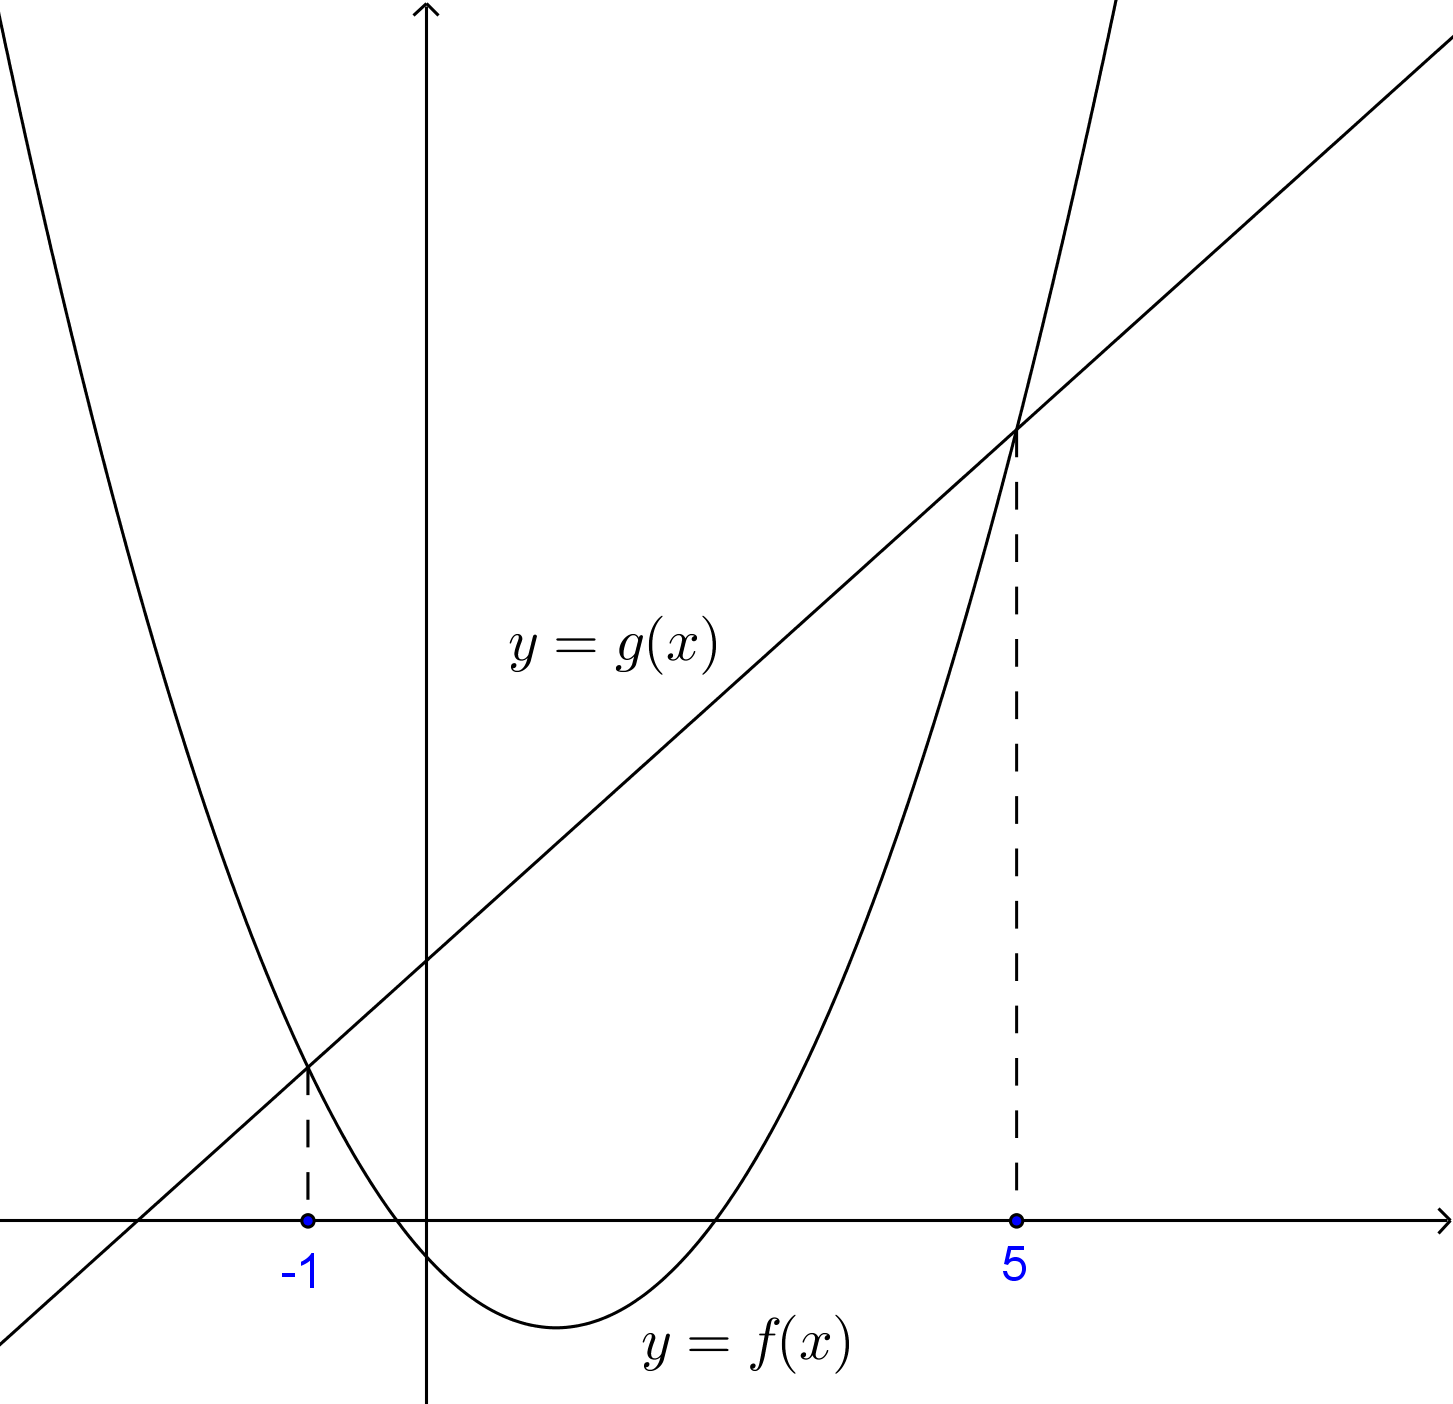
\includegraphics[width=0.5\textwidth]{15}
\end{figure}
\tabb{-7}{-5}{-3}{-1}{1}

%
\prob{19번}
수열 \(\{a_n\}\)은 \(a_1+a_2=8\)이고
\[
\sum_{k=2}^na_k-\sum_{k=1}^{n-1}a_k=n^2\quad(n\ge2)\]
를 만족시킨다.
\(\displaystyle\sum_{k=1}^{10}a_k\)의 값은?
\tabb{388}{392}{396}{400}{404}

\clearpage
%
\prob{20번}
집합 \(X=\{1,2,3,4\}\)에 대하여 \(X\)에서 \(X\)로의 일대일 대응인 함수 \(f\)가 다음 조건을 만족시킨다.
\begin{mdframed}
(가) 집합 \(X\)의 모든 원소 \(x\)에 대하여 \((f\circ f)(x)=x\)이다.\\
(나) 집합 \(X\)의 어떤 원소 \(x\)에 대하여 \(f(x)=5-2x\)이다.
\end{mdframed}

<보기>에서 옳은 것만을 있는 대로 고른 것은?
\begin{mdframed}[frametitle=<보기>]
ㄱ. \(f(2)=f^{-1}(2)\)\\
ㄴ. \(f(2)=2\)이면 \(f(4)=4\)이다.\\
ㄷ. 가능한 함수 \(f\)의 개수는 \(4\)이다.
\end{mdframed}
\tabb{\text{ㄱ}}{\text{ㄴ}}{\text{ㄱ, ㄴ}}{\text{ㄱ, ㄷ}}{\text{ㄱ, ㄴ, ㄷ}}

\clearpage
%
\prob{26번}
전체집합 \(U=\{1,2,3,4,5,6,7\}\)의 두 부분집합
\[A=\{1,3,5,7\},\quad B=\{2,3,4,5\}\]
에 대하여 집합 \(P\)를
\[P=(A\cap B^c)\cup(A^c\cap B)\]
이라 하자.
\(P\subset X\subset U\)를 만족시키는 집합 \(X\)의 개수를 구하시오.
\tabb{2}{4}{8}{16}{32}
%8
\vspace{0.2\textheight}

%
\prob{27번}
\(\displaystyle\sqrt{\frac25}\times\sqrt[4]a\)가 자연수가 되도록 하는 자연수 \(a\)의 최솟값을 구하시오.
%100

\clearpage
%
\prob{28번}
그림과 같이 좌표평면에서 세 점 \(O(0,0)\), \(A=(12,0)\), \(B(0,5)\)를 꼭짓점으로 하는 삼각형 \(OAB\)를 평행이동한 도형을 삼각형 \(O'A'B'\)이라 하자.
점 \(A'\)의 좌표가 \((8,7)\)일 때, 삼각형 \(O'A'B'\)에 내접하는 원의 방정식은 \(x^2+y^2+ax+by+c=0\)이다.
\(a+b+c\)의 값을 구하시오.
(단, \(a\), \(b\), \(c\)는 상수이다.)
\begin{figure}[h!]
\centering
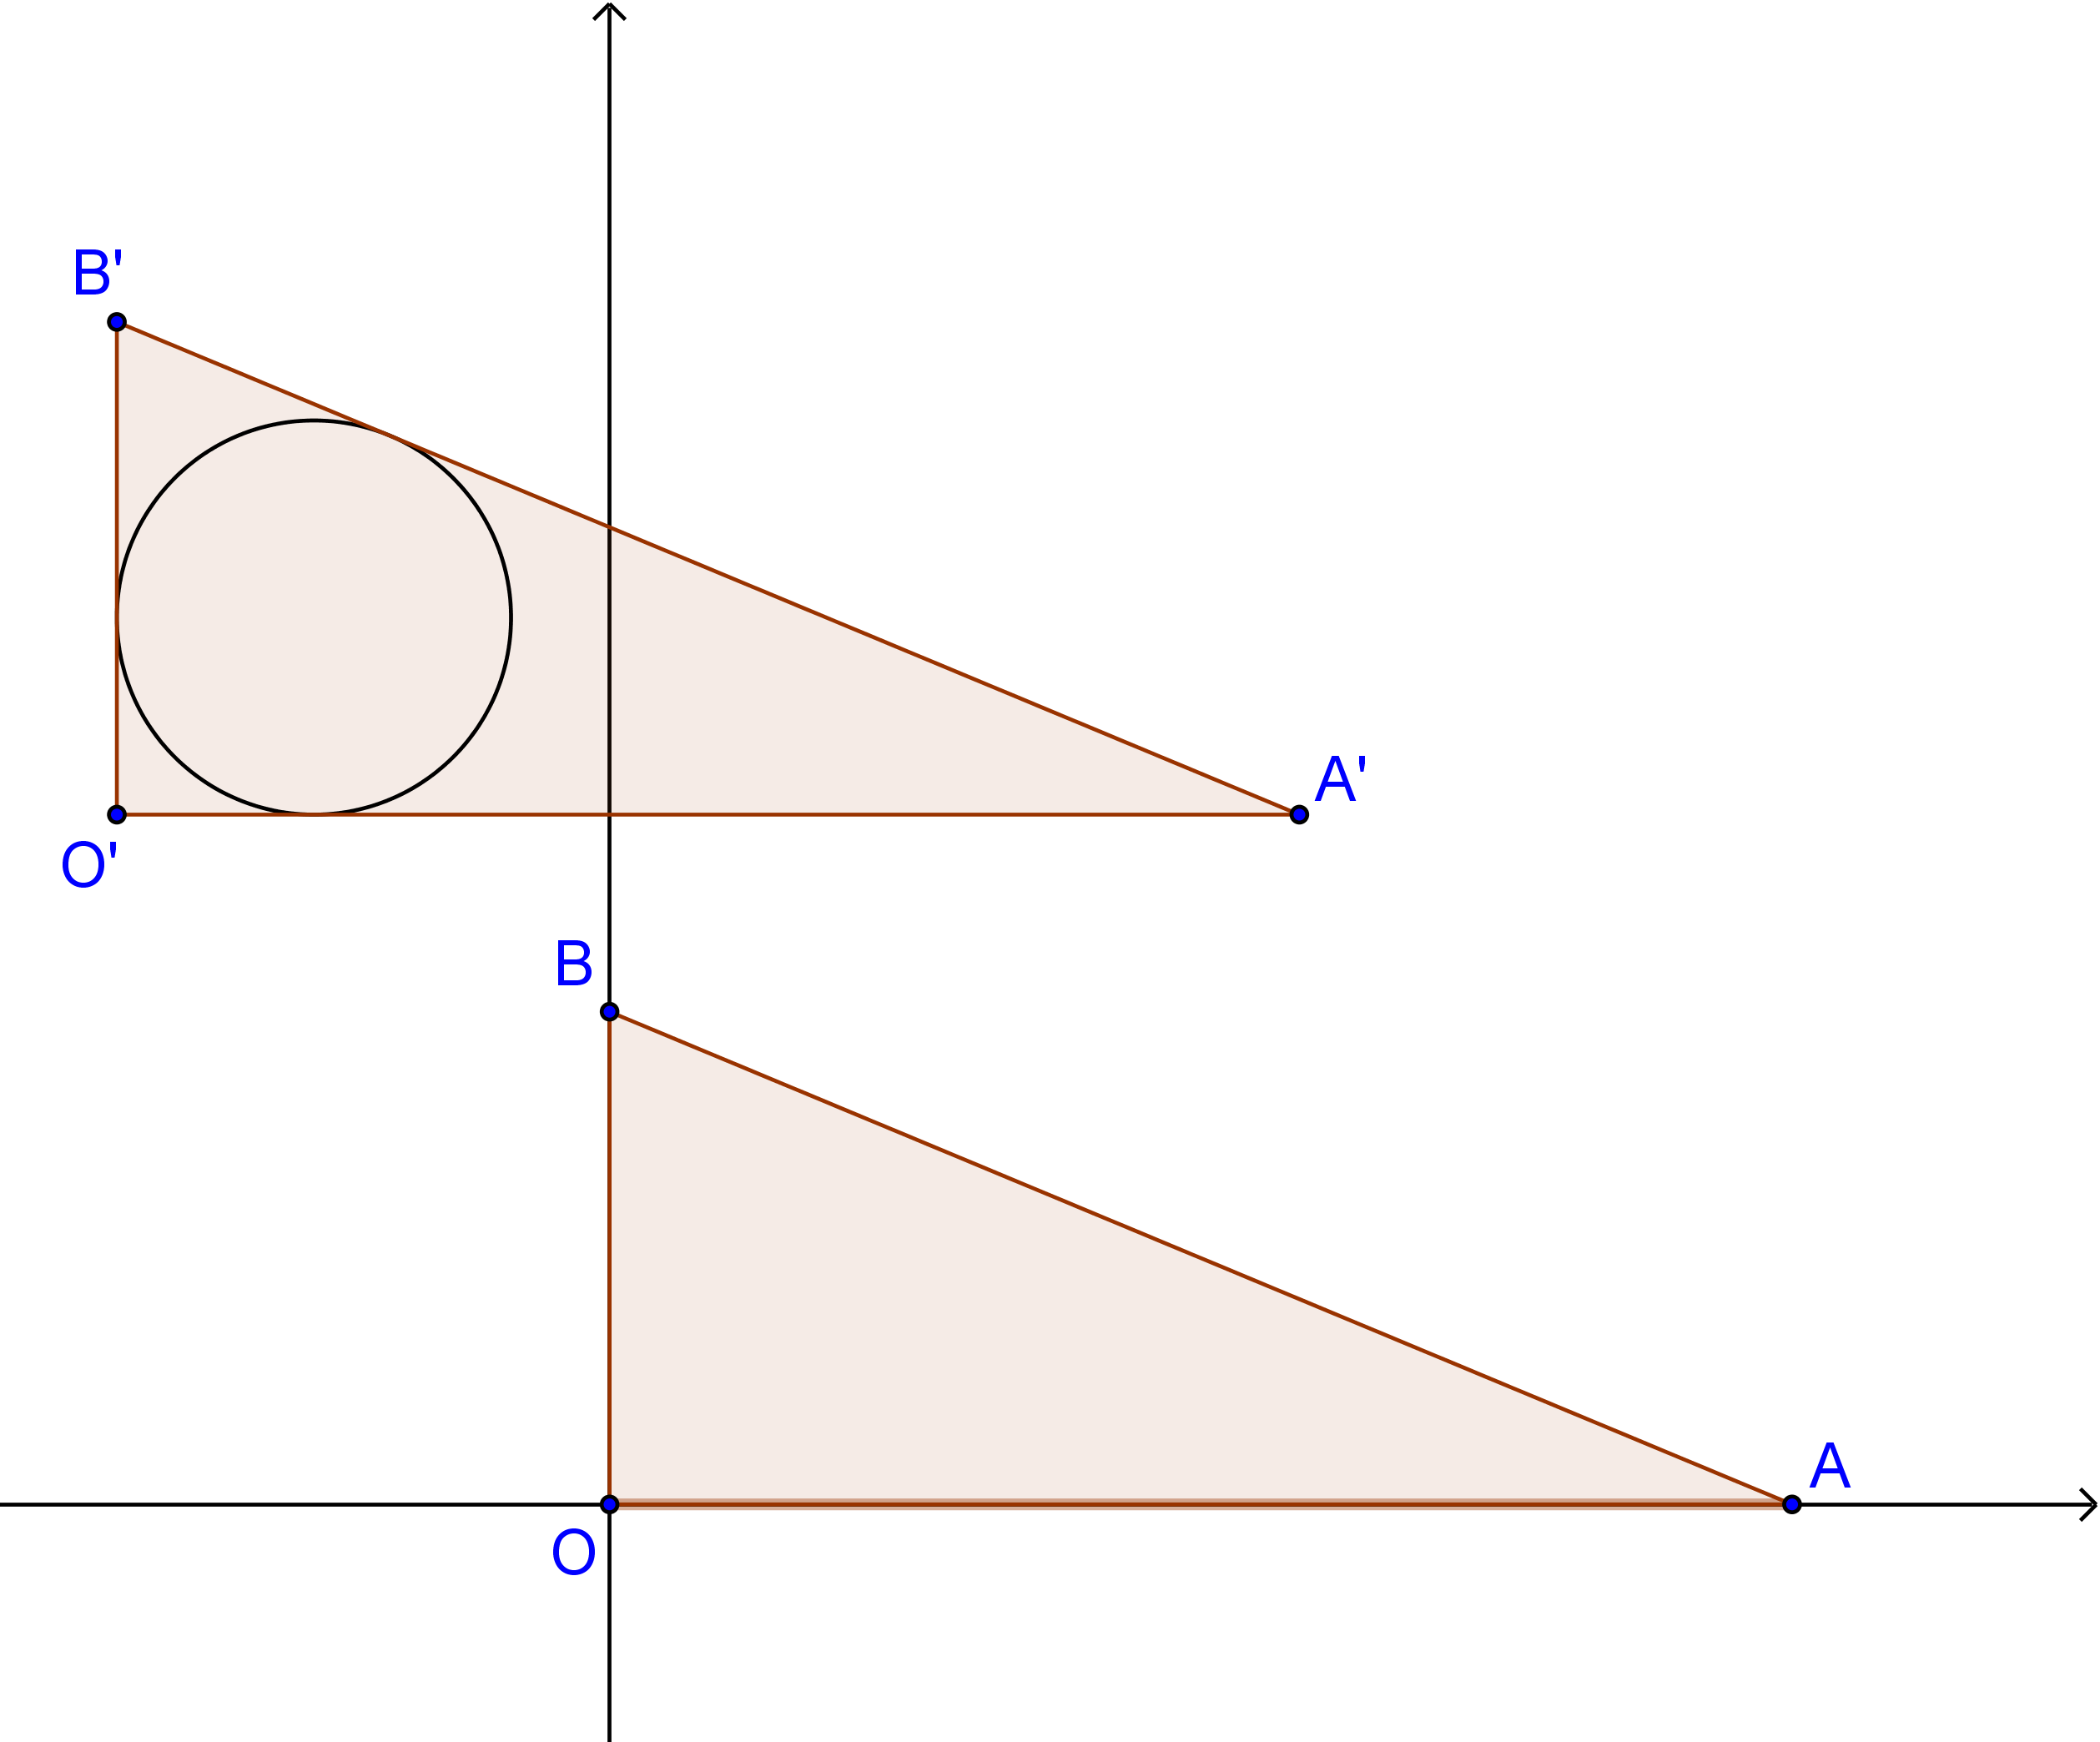
\includegraphics[width=0.5\textwidth]{28}
\end{figure}

\clearpage
%
\prob{29번}
모든 실수 \(x\)에 대하여 이차부등식 \(x^2+2(a-2)x-b^2+2b+1\ge0\)이 성립할 때, \(a+b\)의 최솟값은 \(m\)이다.
\(10m\)의 값을 구하시오.
(단, \(a\), \(b\)는 상수이다.)
%50

\clearpage
%
\prob{30번}
두 등차수열 \(\{a_n\}\), \(\{b_n\}\)과 실수 전체의 집합의 두 부분집합
\begin{align*}
A&=\left\{a_k\ba1\le a_k\le 30,\:a_k\text{는 수열 \(\{a_k\}\)의 항}\right\}\\
B&=\left\{b_k\ba1\le b_k\le 30,\:a_k\text{는 수열 \(\{b_k\}\)의 항}\right\}
\end{align*}
다음 조건을 만족시킨다.
\begin{mdframed}
(가) \(a_1=3\), \(a_{10}=30\)\\
(나) \(n(A\cap B)=n(A\cap B^c)=\frac12\times n(A^c\cap B)\)\\
(다) 집합 \(A\cap B\)의 모든 원소의 합은 \(75\)이다.
\end{mdframed}
집합 \(B\)의 모든 원소의 합을 구하시오.
(단, 수열 \(\{b_n\}\)의 항은 유한개가 아니다.)

\clearpage
%%
\section*{답}
\begin{tabu}spread 50pt{|X[c]|X[c]|X[c]|X[c]|X[c]|}
\hline
1&2&3&4&5\\\hline
\ding{175}&\ding{172}&\ding{176}&\ding{176}&\ding{174}\\\hline
6&7&8&9&\\\hline
\(100\)&\(74\)&\(50\)&\(225\)&\\\hline
\end{tabu}

\end{document}